119. \begin{figure}[ht!]
\center{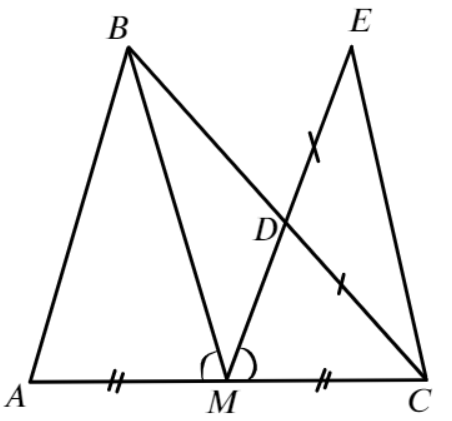
\includegraphics[scale=0.35]{g119.png}}
\end{figure}\\
Продлим $MD$ так, чтобы $DE=DC.$ Тогда $BM=CD+DM=DE+DM=ME.$\\ $\left.\begin{array}{l}BM=ME,\\
AM=MC,\\
\angle BMA=\angle DMC. \end{array}\right\}\Rightarrow \Delta EMC=\Delta BMA\text{ по I признаку.}$ Тогда
$\angle BAC=\angle ECM=\angle ECD+\angle DCM=\angle CEM+\angle ACB=\angle ABM+\angle ACB,$ ч.т.д. $(\angle ECD=\angle CEM$ так как треугольник $CDE$ равнобедренный)\\
